\section{Related Work}
\subsection{SOMs}
\begin{frame}{The GEO SOM}
  \begin{block}{GEO SOM}
    \begin{itemize}
      \item Applies the first law of geography “Everything is related to everything else, but near things are more related than distant things".
      \item  Defining a variable $k$ which is used as a ``geographical tolerance" that forces the winning neuron to be geographically near the input pattern.
      \item selection of the winning neuron is done in two steps. First, geographic neurons inside the tolerance $k$ with the input data as a center are selected. Only after that, comparisons are made with the rest of data present in the input data.
    \end{itemize}
  \end{block}
\end{frame}
\note[itemize]{
      \item Applies the first law of geography “Everything is related to everything else, but near things are more related than distant things".
      \item  Defining a variable $k$ which is used as a ``geographical tolerance" that forces the winning neuron to be geographically near the input pattern.
      \item selection of the winning neuron is done in two steps. First, geographic neurons inside the tolerance $k$ with the input data as a center are selected. Only after that, comparisons are made with the rest of data present in the input data.
}

\begin{frame}{WEBSOM}
  \begin{block}{The WEBSOM self organizing maps}
    \begin{itemize}
      \item  First SOM is called \textit{word category map}  used to find words that have similar meaning.
      \item Second SOM, called \textit{text},  used to cluster the documents.
    \end{itemize}
  \end{block}
\end{frame}
\note[itemize]{
\item by Honkela
\item Websom is used to cluster webpages
\item has two soms
}

\subsection{Twitter}
\begin{frame}{Twitter Natural Language Processing}
  \textbf{ARK Tweet NLP:}
  \begin{itemize}
    \item Built using a maximum entropy Markov model.
    \item Tags words, such as nouns, verbs, etc..
    \item Can tag words, such as abbreviations, emojis and spelling errors. 
  \end{itemize}
  \textbf{Example:}
  \begin{figure}[htpb]
    \centering
    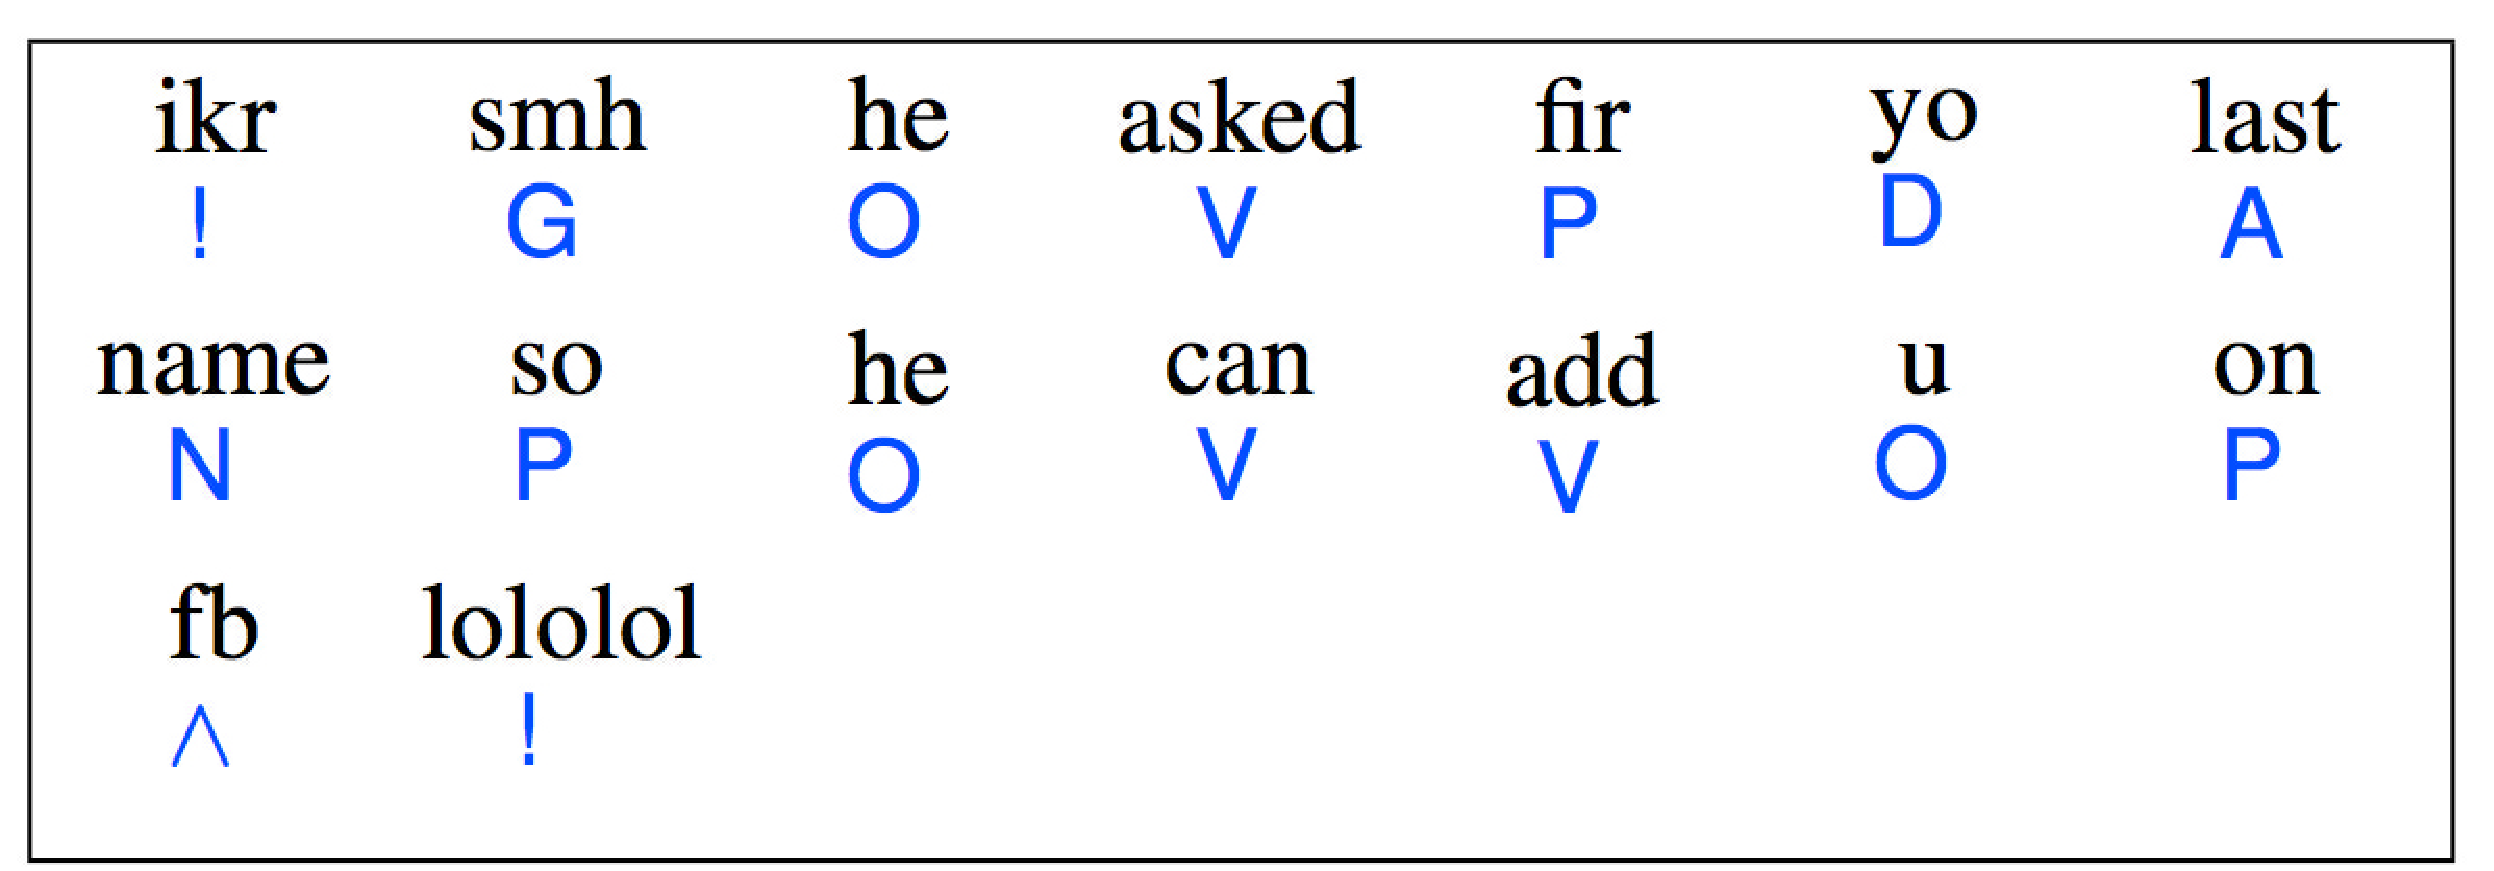
\includegraphics[width=0.6\linewidth]{./images/1_nlp.pdf}
    \label{fig:nlp}
  \end{figure}
\end{frame}
\note[itemize]{
\item Twitter sucks with graphical errors 
\item NLP no twitter antes deste trabalho nao era possivel
  \item Tweet automatically tagged with ARK Tweet NLP. ! stands for interjection, while V stands for verbs and D for determiner.
}

\begin{frame}{Homophily in Social Networks}
  \begin{block}{Miller et al, 2001}
    \begin{itemize}
      \item Similarity breeds connection.
      \item Homophily means \textit{“people like us}.
      \item In diverse societies, race, and race-like ethnicity create the most stark divides.
      \item Sex, age, religion, and education strongly structure our relations with others.
    \end{itemize}
  \end{block}
\end{frame}
\note[itemize]{
\item Not web social, like real social
}
